\chapter[Shallow Water Model]{Shallow Water Model}
\label{chapter:3}

As a first step of investigating how ocean circulation models can be solved using the adaptive wavelet method, the shallow water model was studied.  This 2D model is a simplified version of the full oceanic primitive equations.  

\section{Physical Model and Governing Equations}

The shallow water model is derived from depth averaging the hydrostatic primitive equations under the assumption that the vertical length scale is much smaller than the horizontal length scale (details in Section \ref{derivegoverningeqns}).  Therefore, there is no stratification. 
%
\begin{equation}\label{e:swe_continuity}
\frac{\partial \eta}{\partial t} = -\nabla \cdot (\eta {\bf u})
\end{equation}

\begin{equation*} \label{e:swe_momentum}
\frac{\partial {\bf u}}{\partial t} + {\bf u} \cdot \nabla {\bf u} + \frac{1}{Ro} f \hat{\bf k} \times {\bf u} = - \frac{1}{Fr^2} \nabla \eta
\end{equation*}
%
where $\eta$ is the sea surface height, $u$ and $v$ are the horizontal components of velocity, $f$ is the Coriolis force, $Ro$ is the Rossby number and $Fr$ is the Froud number.  

The free surface allows for propagation of gravity waves, which travel at $c=\sqrt{gH}$.  These are equivalent to acoustic waves in the compressible gas dynamic equations.  

\section{Brinkman Penalization Method for Shallow Water Model}

The shallow water equations are mathematically equivalent to the Euler equations.  A compressible formulation of Brinkman penalization was developed by Liu and Vasilyev \cite{06LV}.  This compressible form was extended to the shallow water equations, 
%
\begin{equation}\label{e:swe_continuity_bp}
\frac{\partial \eta}{\partial t} = - [1+(\frac{1}{\phi}-1)\chi] \nabla \cdot (\eta {\bf u})
\end{equation}

\begin{equation*} \label{e:swe_momentum_bp}
\frac{\partial {\bf u}}{\partial t} + {\bf u} \cdot \nabla {\bf u} + \frac{1}{Ro} f \hat{\bf k} \times {\bf u} = - \frac{1}{Fr^2} \nabla \eta - \frac{\chi}{\eta_{pen}} {\bf u}
\end{equation*}
%
where the Brinkman penalization parameter, $\eta_{pen} \ll 1$ and the porosity parameter, $\phi \ll 1$.  And where, 
%
\begin{equation*} \label{e:chi}
\chi ({\bf x},t) = \left \{ \begin{array}{l} 1 \; \mbox{ if } {\bf x} \in O({\bf x}), \\ 0 \; \mbox{ otherwise}
\end{array} \right \}
\end{equation*}
%
where $O({\bf x})$ is some obstacle or in the case of oceans, land or the ocean floor.

Since the shallow water equations are mathematically similar to the compressible gas dynamic equations, the extension seemed straight-foward.  However, after thorough analysis of the equations and numerical testing, it was found that there are three main differences between the shallow water equations and the gas dynamics equations.  These differences results in a slightly different treatment of the penalization parameters and numerical set up.  

The following analysis describes these differences, while also going through the amplitude and phase error analysis for the case of gravity wave propagation in the small amplitude limit.  

\subsection{Wave Speeds}

One of the assumptions that is made when doing the error analysis for compressible Brinkman penalization was the speed of sound was the same in the fluid region and porous media region.  It was found for the penalized shallow water equations, the gravity wave speed was different in the fluid versus the porous media.  Let's consider the one dimensional shallow water equations,
%
\begin{equation} \label{e:1dswe}
\frac{\partial {\bf u}}{\partial t} + {\bf A} \frac{\partial{\bf u}}{\partial x} = 0
\end{equation}
%
where ${\bf u}=(\eta, \eta u)^{T}$ is the vector of conservative, dimensional variables and the Jacobian matrix is, 
%
\begin{equation*}
{\bf A} = \left[ \begin{array}{cc}
0 & \frac{1}{\phi} \\
g \eta - \frac{(\eta u)^2}{\eta^2} & \frac{2 (\eta u)}{\eta} \end{array} \right]
\end{equation*}
%
Note that when $\phi =1$, the equations reduce to the traditional shallow water equations.  Therefore, $\phi=1$ represents the fluid case, while all other cases are for the porous media.  To find the gravity wave speed in both regions, the eigenvalues of the Jacobian matrix, ${\bf A}$, can be found by solving, 
%
\begin{equation*}
|{\bf A} - \lambda {\bf I}|=0
\end{equation*}
%
which gives, 
%
\begin{equation*}
\lambda^2 - 2 u \lambda + \frac{1}{\phi} (u^2 - g \eta)=0
\end{equation*}
%
solving for the roots, 
%
\begin{equation} \label{e:lambda}
\lambda = u \pm \sqrt{u^2 - \frac{1}{\phi} (u^2 - g \eta)}
\end{equation}
%
With some scale analysis, Equation \ref{e:lambda} can be simplified.  Assuming that $u~\phi$ and $\eta = H + \epsilon$, where $H$ is the mean depth of the ocean and $\epsilon$ is some small perturbation ($\epsilon \ll H$).  Thus, the eigenvalues become,  
%
\begin{equation} \label{e:eigenvalues}
\lambda = u^2 \pm \sqrt{\frac{gH}{\phi}}
\end{equation}
%
When $\phi =1$, the eigenvalues are $u \pm \sqrt{gH}$, as expected for shallow water gravity wave speed.  However, for the any other $\phi$ value, the eigenvalues are not the same.  Since $\phi \ll 1$ for the Brinkman penalization formulation, the gravity wave speed inside the porous media is much larger than that in the fluid region.  

\subsection{Impedance}

This section looks at some properties associated with the classical theory of acoustics \cite{00Blackstock} that were used in the development of the compressible formulation of Brinkman penalization \cite{06LV}.  Thus, consider the plane wave refelction and transmission at the interface between two different media.  To model the one dimensional problem of wave progragation in a fluid to porous media, it can be though of us a sudden change in cross-sectional area.  From the acoustics theory, the acoustic impedance at a given surface is the ratio of the surface-averaged acoustic pressure to the fluid volume velocity,  
%
\begin{equation*}
Z=\frac{\rho c}{S}
\end{equation*}
%
where $\rho$ is density, $c$ is gravity wave speed in the fluid ($c=\sqrt{gH}$), and $S$ is the cross-sectional area.  In order to have most of the wave reflected, the obstacle's acoustic impedance needs to be sufficiently large, the basis for Impedance Mismatch Method \cite{95Chung}.  For the case of the shallow water equations, since the gravity wave speed is also a function of $\phi$, the impedance becomes, 
%
\begin{equation*}
Z=\frac{\rho c}{\phi ^{3/2}}
\end{equation*}
%
which is a higher impedance than what was found for the compressible Brinkman penalization formulation, which was $Z=\frac{\rho c}{\phi}$.  This allows for a slightly lower range of reasonable $\phi$ values allowed for negligible wave transmission in the shallow water case over the compressible gas case.    This is a nice feature of this extension of Brinkman penalization.  

\subsection{Amplitude and Phase Errors by Asymptotic Analysis}

The use of asymptotic analysis will provide a way to estimate the amplitude and phase errors associated with the penalized shallow water equations.  In addition, by looking at the equations in different asymptotic limits, it provides information about the behavior of the system from a rigorous mathematical viewpoint.  The following analysis is assumes small amplitude waves in the ocean region and was derived from work done on the penalized compressible gas dynamic equations \cite{06LV}.  

\subsubsection{Asymptotic Analysis for Ocean Region}

For the ocean region, the variables can be written as, 
%
\begin{equation} \label{e:oceanregionterms1}
\eta_{\rm o} = 1 + \epsilon \eta_{\rm o}^{\prime}
\end{equation}

\begin{equation} \label{e:oceanregionterms2}
u_{\rm o} = \epsilon u_{\rm o}^{\prime}
\end{equation}
%
where $\epsilon \ll 1$.  If Equations \ref{e:oceanregionterms1} and \ref{e:oceanregionterms2} are substituted into Equations \ref{e:swe_continuity_bp} and \ref{e:swe_momentum_bp} and only the leading perturbation terms are kept, the result is a wave equation, 
%
\begin{equation} \label{e:waveeqn_eta}
\frac{\partial ^2 \eta_{\rm o}^{\prime}}{\partial t^2} = \frac{\partial ^2 \eta_{\rm o}^{\prime}}{\partial x^2}
\end{equation}

\begin{equation} \label{e:waveeqn_u}
\frac{\partial ^2 u_{\rm o}^{\prime}}{\partial t^2} = \frac{\partial ^2 u_{\rm o}^{\prime}}{\partial x^2}
\end{equation}

\subsubsection{Asymptotic Analysis for Continental Region}

For the continental region, the variables can be written as, 
%
\begin{equation} \label{e:contregionterms1}
\eta_{\rm c} = 1 + \epsilon \eta_{\rm c}^{\prime}
\end{equation}

\begin{equation} \label{e:contregionterms2}
u_{\rm c} = \epsilon \eta_{pen} u_{\rm c}^{\prime}
\end{equation}
%
The leading perturbation terms in this case are different from the ocean region because of the strong Brinkman damping term in the momentum equation.  If Equations \ref{e:contregionterms1} and \ref{e:contregionterms2} are substituted into Equations \ref{e:swe_continuity_bp} and \ref{e:swe_momentum_bp} and only the leading order terms are kept, the result is a diffusion equation, 
%
\begin{equation} \label{e:diffeqn_eta}
\frac{\partial \eta_{\rm c}^{\prime}}{\partial t} = \alpha \frac{\partial ^2 \eta_{\rm c}^{\prime}}{\partial x^2}
\end{equation}

\begin{equation} \label{e:diffeqn_u}
\frac{\partial u_{\rm c}^{\prime}}{\partial t} =\alpha \frac{\partial ^2 u_{\rm c}^{\prime}}{\partial x^2}
\end{equation}
%
where $\alpha=\frac{\eta_{pen}}{\phi}$.  

\subsubsection{Asymptotic Analysis for Boundary Layer}

The asymptotic analysis for the ocean and continental region is only valid away from the interface, because of the length and magnitude scales of the perturbations used.  For the boundary layer, the variables can be written as, 
%
\begin{equation} \label{e:blregionterms1}
\eta_{\rm bl} = 1 + \epsilon \eta_{\rm bl}^{\prime}
\end{equation}

\begin{equation} \label{e:blregionterms2}
u_{\rm bl} = \epsilon \eta_{pen} u_{\rm bl}^{\prime}
\end{equation}

If Equations \ref{e:blregionterms1} and \ref{e:blregionterms2} are substituted into Equations \ref{e:swe_continuity_bp} and \ref{e:swe_momentum_bp} and only the leading order terms are kept, the result is a diffusion equation, 
%
\begin{equation} \label{e:diffeqn_eta_bl}
\frac{\partial \eta_{\rm bl}^{\prime}}{\partial t} = \alpha \frac{\partial ^2 \eta_{\rm bl}^{\prime}}{\partial x^2}
\end{equation}

\begin{equation} \label{e:diffeqn_u_bl}
\frac{\partial u_{\rm bl}^{\prime}}{\partial t} =\alpha \frac{\partial ^2 u_{\rm bl}^{\prime}}{\partial x^2}
\end{equation}

This is where the penalized shallow water equations differ greatly from the penalized compressible gas dynamic equations.  For the compressible gas dynamic equations, it was found that there was a boundary layer region that transitioned the two other asymptotic solutions nicely \cite{06LV}.  Therefore, in addition to the fluid region being governed by the acoustic wave equation and the porous media region being governed by a diffusion equations, there exists a boundary layer region in between that is governed by a diffusive wave equation.  This boundary layer does not exist in the penalized shallow water equations.  It has been shown here, that the boundary layer is the same as the continental region, leaving no natural, mathematical transition.  As a result, numerical techniques need to be employed to create that transition to maintain numerical stability.  

Additionally, it was found for the compressible gas dynamic formulation that it wasn't necessary to resolve the boundary layer.  For the shallow water formulation, it is necessary to resolve the numerical boundary layer.  This makes it slightly more expensive.  However, since the shore of the ocean is not necessarily a solid wall, it seems that modeling it as a slightly gradual change from fluid to solid may result is a more accurate representation.  It does not seem necessary to have a sharp transition.  As a result, the computational cost can be minimized.  Either way, the theory works in the limit of a solid wall given the proper computational resources.  

\section{Benchmark Problem I: One Dimensional normal wave}

To verify convergence of the method, a one dimensional test case was used.  A one dimensional normal wave was initialized for the sea surface height.  The velocity was initialized to zero, as shown in Figure \ref{f:initial_wave}.  

\begin{center}
 \begin{figure}[h!]
\centering
\subfigure{
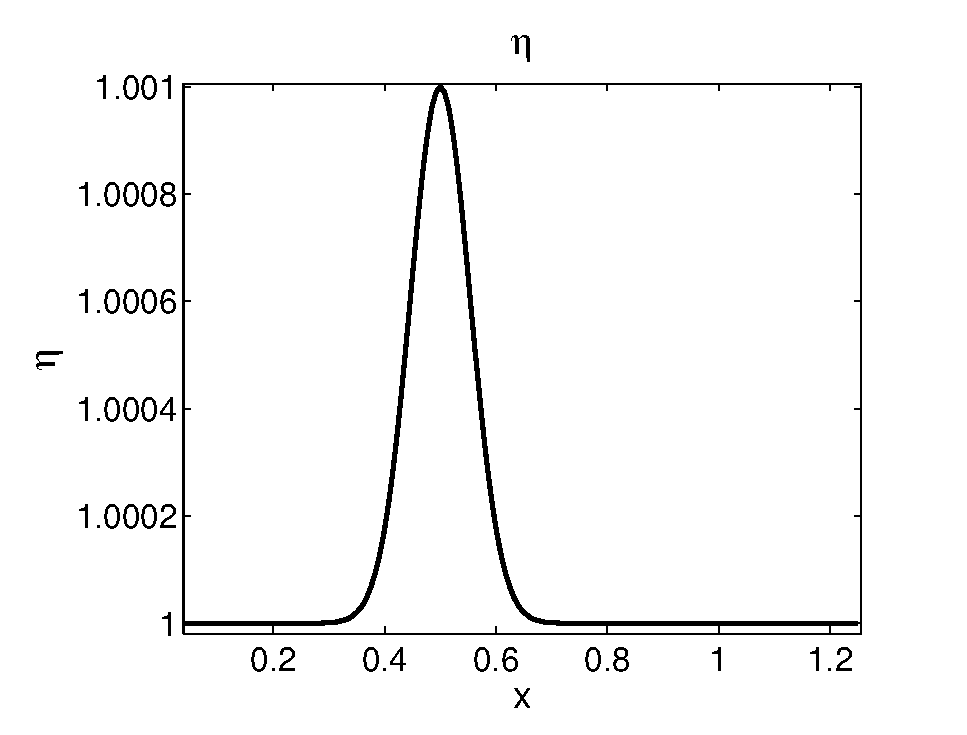
\includegraphics[scale=.4]{Images/initial_eta}
}
\subfigure{
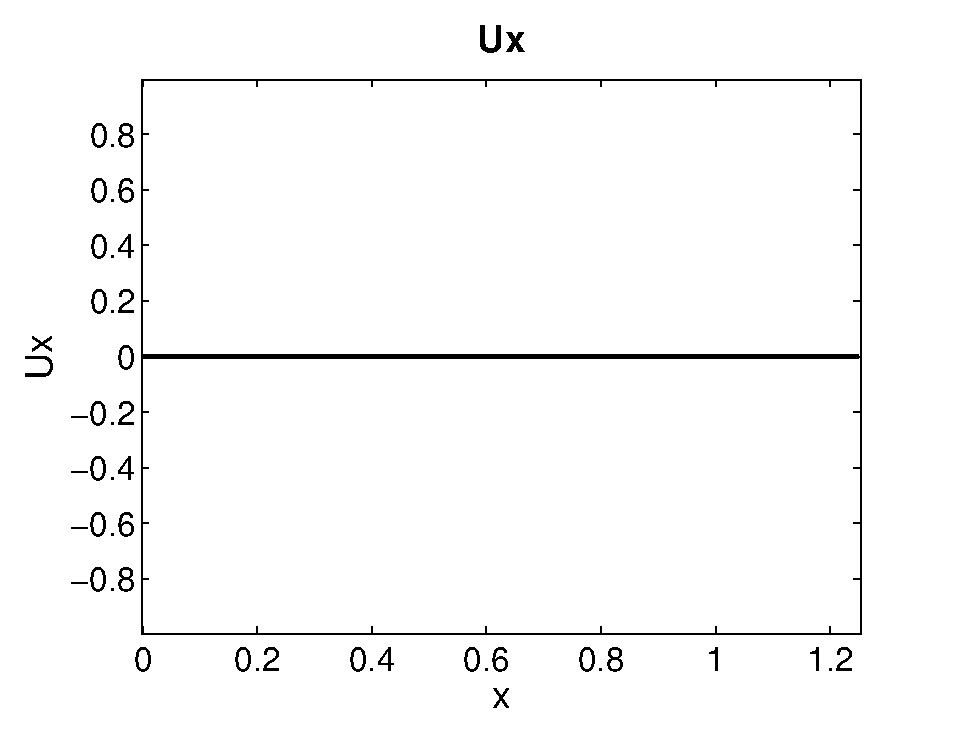
\includegraphics[scale=.4]{Images/initial_ux}
}
\caption[Initial conditions for 1D wave ]{Initial conditions for 1D wave.}
\label{f:initial_wave}
\end{figure}
\end{center}

The wave splits and propagates to the east and west.  On the east side, it hits a Brinkman zone and on the west side, it hits a regular no slip boundary wall.  This allowed for comparison between the two methods.  After complete reflection, the solution is shown in Figure \ref{f:reflected_wave}.  

\begin{center}
 \begin{figure}[h!]
\centering
\subfigure{
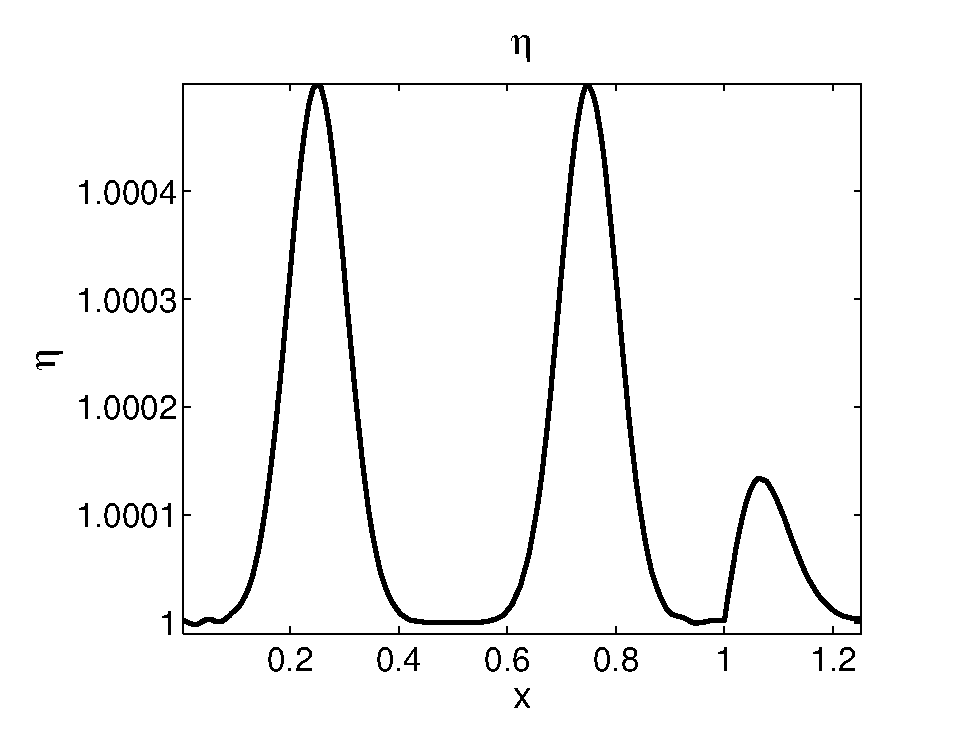
\includegraphics[scale=.4]{Images/reflection_eta}
}
\subfigure{
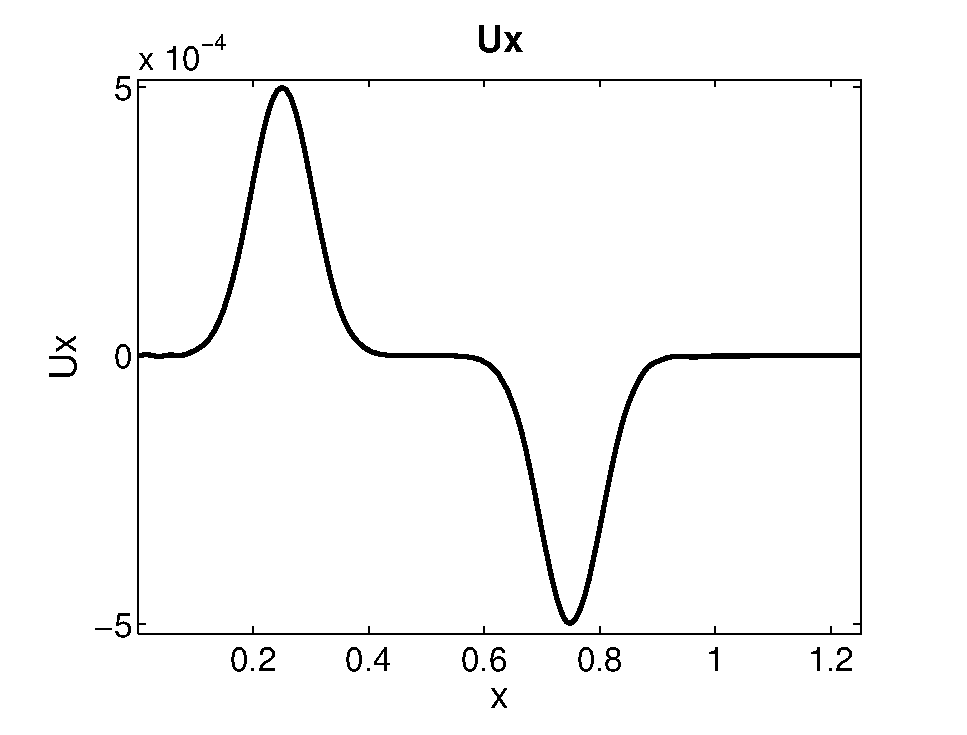
\includegraphics[scale=.4]{Images/reflection_ux}
}
\caption[ 1D wave after complete reflection]{1D wave after complete reflection.}
\label{f:reflected_wave}
\end{figure}
\end{center}

Figure \ref{f:reflected_wave} not only demonstrates how the no slip boundary conditions are satisfied on the Brinkman wall, but also shows the decaying solution for sea surface height in the Brinkman zone.  The small decay solution is negligible because it is actually multiplied by $\phi$.  

\begin{center}
\begin{figure}[h!]
\centering
  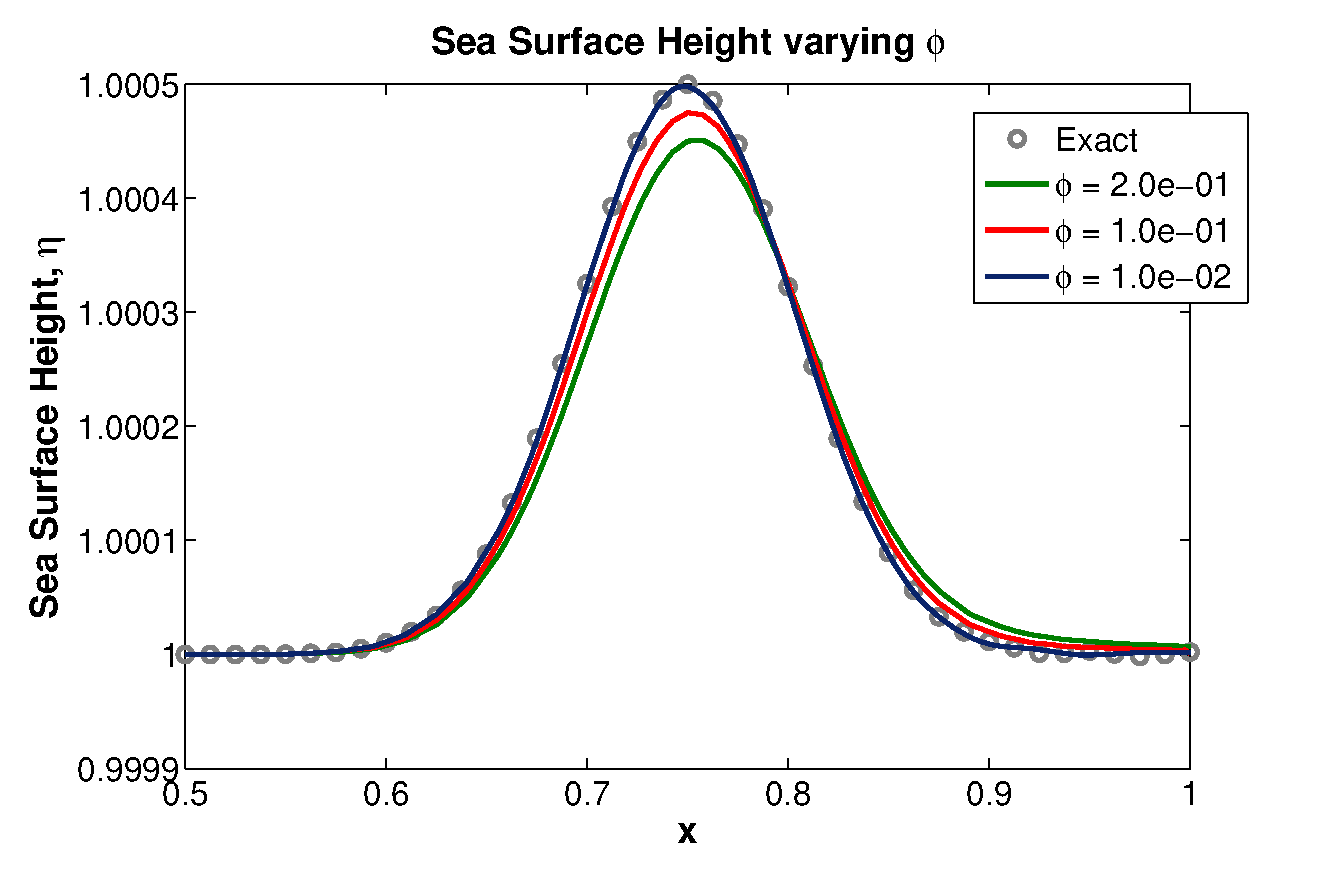
\includegraphics[width=4in]{Images/etaconvergence}
  \caption[Sea surface height convergence plot]{Plot of sea surface height for various porosity parameters.}\label{f:etaconvergence}
\end{figure}
\end{center}

\begin{center}
\begin{figure}[h!]
\centering
  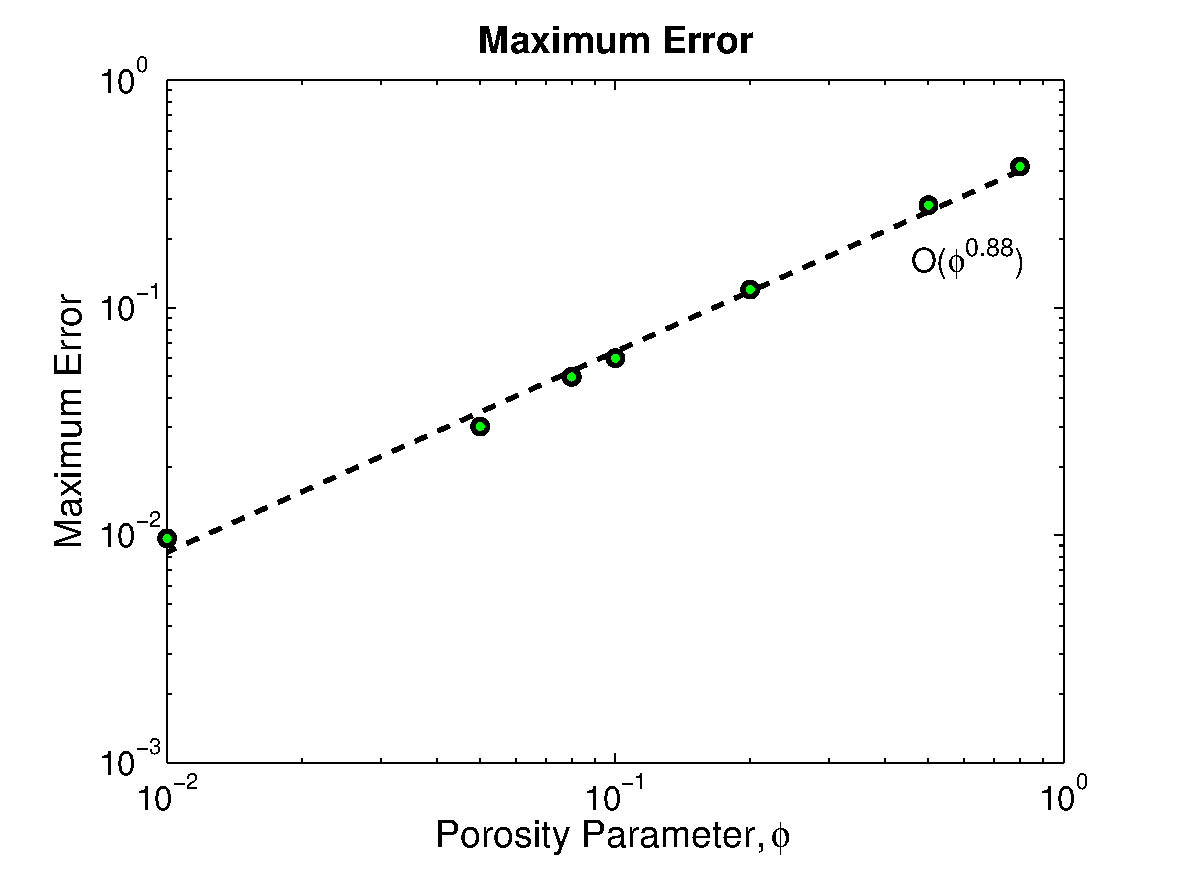
\includegraphics[width=4in]{Images/maxerrorconvergence}
  \caption[Maximum error convergence plot.]{Plot of max error versus porosity parameter, $\phi$, which demonstrates convergence of $O(0.88)$}\label{f:maxerrorconvergence}
\end{figure}
\end{center}


\section{Two-dimensional Wind-driven Double Gyre with Brinkman}

Various 2D studies have been done to verify the new formulation of Brinkman penalization.  First, a 2D wind-driven double gyre test case was run on a rectangular domain.  This was done with traditional no-slip boundary conditions in one case and with Brinkman penalization (and straight boundaries) in another case.  These two cases compare nicely visually, as can be seen in Figure \ref{f:2D_swe_bpresults}.  Further work needs to be done to more thoroughly analyze these 2D results.

\begin{center}
\begin{figure}[h!]
\centering
  \includegraphics[width=6in]{Images/2D_swe_bpresults}
  \caption[2D wind-driven results with Brinkman]{2D plots of sea surface height, velocity, and the adaptive grid for a wind-driven double gyre circulation using Brinkman penalization.}\label{f:2D_swe_bpresults}
\end{figure}
\end{center}

Initial studies of variable topography have also been done.  This cannot be compared to traditional boundary conditions, but can verify the stability of the method. There is a short transient time for this steady state solution to adjust to the Brinkman penalization.  This is the case for a rectangular domain, as well.  It takes the solution a slightly longer to adjust for a non-rectangular domain.  However, if one could start with better initial conditions, then this can be avoided.  Since, we are interested in a steady state solution, this is not an issue.  

\begin{center}
\begin{figure}[h!]
\centering
  \includegraphics[width=6in]{Images/2D_swe_bpvaryresults}
  \caption[2D wind-driven results with Brinkman for variable topography]{2D plots of velocity and the adaptive grid for a wind-driven double gyre circulation using Brinkman penalization for variable topography.}\label{f:2D_swe_bpvaryresults}
\end{figure}
\end{center}

